\begin{abox}
	Assignment-S05\\
	\vspace{0.5cm}
	Motion of Charged Particle in Uniform Electric and Magnetic Field
	\end{abox}
\begin{enumerate}
	\item $\left. \right. $
	\begin{answer}
		\begin{align*}
		\text{(a) Acceleration of the particle is }a&=\frac{q E}{m}=\frac{q}{m}\left(E_{0}-a x\right)\\
		\text{The equation of motion is, }\frac{d v}{d t}&=v \frac{d v}{d x}=\frac{q}{m}\left(E_{0}-a x\right)\\
		\text{Integrating, }\frac{v^{2}}{2}&=\frac{q}{m}\left(E_{0} x-a \frac{x^{2}}{2}\right)+C.\\
		\because v=0\text{ at }x&=0 \Rightarrow C=0 \Rightarrow v^{2}=\frac{2 q}{m}\left(E_{0} x-a \frac{x^{2}}{2}\right).\\
	\text{	Thus, }v&=0\text{ again at }x=x_{m}=\frac{2 E_{0}}{a}.\\
		\text{(b) The corresponding acceleration is, }\left(\frac{d v}{d t}\right)_{x=x_{m}}&=\frac{q}{m}\left(E_{0}-2 E_{0}\right)=-\frac{q E_{0}}{m}
		\end{align*}
	\end{answer}
\item $\left. \right. $
\begin{answer}
	(a) Assuming that there is no magnetic field, one has from the Lorentz force \\$F=m a=q E=q V / d$, where one neglects gravitational acceleration.\\
	The acceleration is constant, and it is $a=q V /(d m)$.
	\begin{align*}
\text{(b) }y&=\frac{1}{2} a t^{2}\text{ and }x=v t \Rightarrow y=\frac{1}{2} a\left(\frac{x}{v}\right)^{2}=\frac{a}{2 v} x^{2}=\frac{q V}{2 v m d} x^{2}.
\intertext{Thus path is parabolic.}
\text{(c) }y&=0.5 a t^{2} \Rightarrow d y=a t d t\text{ and the fact that }x=L=v t \Rightarrow d x=v d t\text{ and }t=L / v,\\&\text{ one can calculate the angle as }\tan \theta \approx d y / d x=\frac{a t d t}{v d t}=a t / v=\frac{q V L}{v^{2} d m} .\\
&\theta \approx \tan ^{-1}\left(\frac{q V L}{v^{2} d m}\right)
	\end{align*}
\end{answer}
\item $\left. \right. $
\begin{answer}
	 Equating the centripetal force with the Lorentz Force, $m v^{2} / R=q v B$.
	The radius of curvature used in the centripetal force equation is given by
	\begin{align*}
 R^{2}&=l^{2}+(R-s)^{2},\\
	\Rightarrow R^{2}&=l^{2}+(R-s)^{2}=l^{2}+R^{2}+s^{2}-2 R s \approx l^{2}+R^{2}-2 R s+O\left(s^{2}\right) \quad \because s<<l\\
	\Rightarrow l^{2}&=2 R s \Rightarrow R=l^{2} /(2 s) .\\
\text{	Now }m v / R&=q B \Rightarrow 2 s m v / l^{2}=q B \Rightarrow p=m v=q B l^{2} / 2 s,
	\end{align*}
\end{answer}
\item $\left. \right. $
\begin{answer}
	\begin{align*}
K E_{\max }&=\frac{q^{2} B^{2} r^{2}}{2 m} \Rightarrow \frac{K_{p}}{K_{d}}\\&=\left(\frac{q_{p}}{q_{d}}\right)^{2} \times \frac{m_{d}}{m_{p}}=\left(\frac{q}{q}\right)^{2} \times \frac{2 m_{p}}{m_{p}} \Rightarrow K_{p}=2 K_{d}=10 \mathrm{MeV}\\
	\text{(b) }K E_{\max }&=\frac{q^{2} B^{2} r^{2}}{2 m} \Rightarrow \frac{K_{\alpha}}{K_{d}}=\left(\frac{q_{\alpha}}{q_{d}}\right)^{2} \times \frac{m_{d}}{m_{\alpha}}\\&=\left(\frac{2 e}{e}\right)^{2} \times \frac{2 m_{p}}{4 m_{p}} \Rightarrow K_{\alpha}=2 K_{d}=10 \mathrm{MeV}\\
	\text{(c) }f&=\frac{q B}{2 \pi m} \Rightarrow \frac{f^{\prime}}{f_{\alpha}}=\frac{q^{\prime}}{q_{\alpha}} \times \frac{m_{\alpha}}{m^{\prime}}\\&=\frac{q}{q} \times \frac{4 m_{p}}{3 m_{p}}=\frac{4}{3} \Rightarrow f^{\prime}=8 M H z
	\end{align*}
\end{answer}
\item $\left. \right. $
\begin{answer}
	\begin{align*}
R&=\frac{m v}{q B} \Rightarrow R=\frac{\sqrt{2 m K . E}}{q B}\\
	\Rightarrow R_{p}&=\frac{\sqrt{2 m_{p} \times 2 K}}{e B}=\frac{2 \sqrt{m_{p} K}}{e B}, R_{d}=\frac{\sqrt{2 m_{d} \times 4 K}}{e B}\\&=\frac{\sqrt{4 m_{p} \times 4 K}}{e B}=\frac{4 \sqrt{m_{p} K}}{e B} \\
	\text { and } R_{\alpha}&=\frac{\sqrt{2 m_{\alpha} \times 8 K}}{2 e B}=\frac{\sqrt{8 m_{p} \times 8 K}}{2 e B}=\frac{4 \sqrt{m_{p} K}}{e B} \\
	\Rightarrow R_{p}: R_{d}: R_{\alpha}&=2: 4: 4=1: 2: 2
	\end{align*}
\end{answer}
\item $\left. \right. $
\begin{answer}
	\begin{align*}
	\because m v_{n} r_{n}&=n \hbar\text{ and }r_{n}\\&=\frac{m v_{n}}{q B} \Rightarrow r_{n}=\frac{m}{q B} \frac{n \hbar}{m r_{n}} \Rightarrow r_{n}^{2}=\frac{n \hbar}{q B} \Rightarrow r_{n}=\sqrt{\frac{n \hbar}{q B}}\\
	\text{(b) }\because E_{n}&=\frac{q^{2} B^{2} r_{n}^{2}}{2 m} \Rightarrow E_{n}=\frac{q^{2} B^{2} r_{n}^{2}}{2 m}\\&=\frac{q^{2} B^{2}}{2 m} \times \frac{n h}{q B}=n\left(\frac{q B h}{4 \pi m}\right)
	\end{align*}
\end{answer}
\item $\left. \right. $
\begin{answer}
	\begin{align*}
	K E_{\max }&=m c^{2}-m_{0} c^{2}=m_{0} c^{2} \Rightarrow m=2 m_{0}\\
	\because m&=\frac{m_{0}}{\sqrt{1-\frac{v^{2}}{c^{2}}}} \Rightarrow 2 m_{0}=\frac{m_{0}}{\sqrt{1-\frac{v^{2}}{c^{2}}}} \Rightarrow v=\frac{\sqrt{3}}{2} c \\
	\because R&=\frac{m v}{e B} \Rightarrow B=\frac{m v}{e R}=\frac{2 m_{0}}{e R} \frac{\sqrt{3}}{2} c=\frac{\sqrt{3} m_{0} c}{e R}
	\end{align*}
\end{answer}
\item $\left. \right. $
\begin{answer}
	\begin{align*}
	E&=\frac{q^{2} B^{2} R^{2}}{2 m_{p}} \Rightarrow 1.6 \times 10^{-13}=\frac{\left(1.6 \times 10^{-19}\right)^{2} B^{2}(0.1)^{2}}{2\left(1.67 \times 10^{-27}\right)} \Rightarrow B^{2}\\&=\frac{1.6 \times 10^{-13} \times 2\left(1.67 \times 10^{-27}\right)}{\left(1.6 \times 10^{-19}\right)^{2}(0.1)^{2}}\\
	\Rightarrow B^{2}&=\frac{10^{-13} \times 2\left(1.67 \times 10^{-27}\right)}{\left(1.6 \times 10^{-38}\right)(0.01)}=\frac{3.34 \times 10^{-40}}{1.6 \times 10^{-40}}\\&=2.08 \Rightarrow B=\sqrt{2.08}\text{ Tesla $=1.44$ Tesla}
	\end{align*}
\end{answer}
\item $\left. \right. $
\begin{answer}
	\begin{align*}
	\text{Pitch of the helix }l&=v_{\|} T=\frac{v_{\perp}}{2} \frac{2 \pi R}{v_{\perp}}=\pi R \Rightarrow \frac{l}{R}=\pi\\
	\because v_{\|}&=\frac{v_{\perp}}{2}
	\end{align*}
\end{answer}
\item $\left. \right. $
\begin{answer}$\left. \right. $
	\begin{figure}[H]
		\centering
		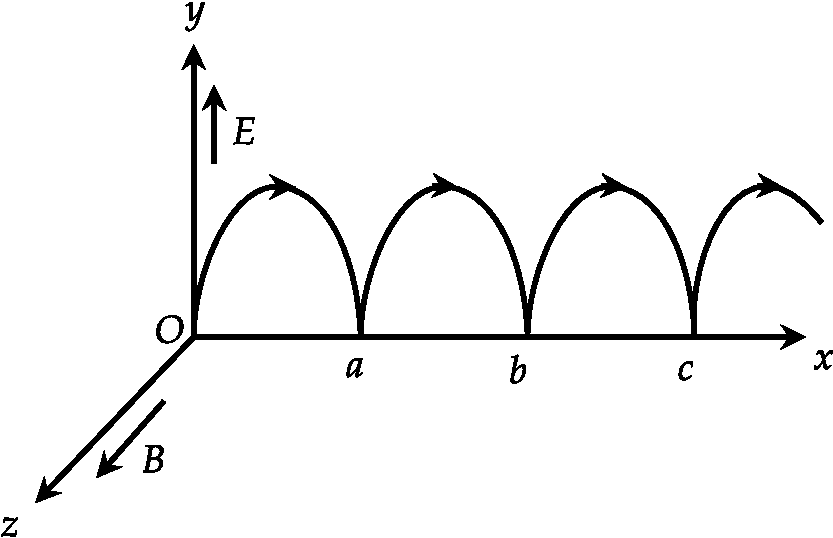
\includegraphics[height=4cm,width=7cm]{Assi-S19}
	\end{figure}
		If $\vec{B}$ points in $z$-direction and $\vec{E}$ points in $y$-direction, and a particle at rest is released from origin, then particle will follow cycloid motion.\\
	Initially, the particle is at rest, so the magnetic force is zero, and the electric field accelerates the charge in $y$-direction. As it speeds up, a magnetic force develops which pulls the charge to the right. The faster it goes stronger the magnetic force becomes and it curves the particle back around towards the $x$-axis. At this point the charge is moving against the electric force, so it begins to slow down-the magnetic force then decreases, and the electrical force takes over, bringing the charge to rest at point $a$ and then process repeats.\\
	(a) Charge particle will confine in a plane that is perpendicular to $\vec{B}$. So it will confine in $x y$-plane.
	\begin{align*}
\text{(b) }\vec{v}&=\dot{x} \hat{x}+\dot{y} \hat{y}\text{ and }\vec{a}=\ddot{x} \hat{x}+\ddot{y} \hat{y}\\
\vec{F}&=q(\vec{E}+\vec{v} \times \vec{B})=q(E \hat{y}+B \dot{y} \hat{x}-B \dot{x} \hat{y})=m \vec{a}=m(\ddot{x} \hat{x}+\ddot{y} \hat{y}) \\
\Rightarrow \ddot{x}&=\omega \dot{y}, \ddot{y}=\omega\left(\frac{E}{B}-\dot{x}\right) \quad \text { where } \omega=\frac{q B}{m}(\text { cylotron frequency })
\intertext{(c) Let us solve the above differential equations,}
\because \ddot{x}&=\omega \dot{y} \Rightarrow \dddot x=\omega \ddot{y} \Rightarrow \dddot x=\omega^{2}\left(\frac{E}{B}-\dot{x}\right) \quad \because \ddot{y}=\omega\left(\frac{E}{B}-\dot{x}\right)\\
\Rightarrow \dddot x+\omega^{2} \dot{x}&=\omega^{2} \frac{E}{B} \\
\text { Let } \dot{x}&=t^{\prime} \Rightarrow \dddot t+\omega^{2} t^{\prime}=\omega^{2} \frac{E}{B}\\
\text{For $C . F$.}&\\
D^{2}+\omega^{2}&=0 \Rightarrow D=\pm i \omega \Rightarrow C . F .=C_{1}^{\prime} \cos \omega t+C_{2}^{\prime} \sin \omega t\\
\text{For $P . I$.}&\\
\text { P.I. }&=\frac{1}{D^{2}+\omega^{2}}\left(\omega^{2} \frac{E}{B}\right)=\frac{1}{0^{2}+\omega^{2}}\left(\omega^{2} \frac{E}{B}\right)=\frac{E}{B}\\
\text{Thus }t^{\prime}&=\dot{x}=C . F .+P . I=C_{1}^{\prime} \cos \omega t+C_{2}^{\prime} \sin \omega t+\frac{E}{B}\\
\Rightarrow x(t)&=C_{1} \sin \omega t+C_{2} \cos \omega t+\frac{E}{B} t+C_{3} \quad \text{ where }C_{1}=\frac{C_{1}^{\prime}}{\omega}, C_{2}=-\frac{C_{2}^{\prime}}{\omega} .\\ \because \omega \dot{y}&=\ddot{x} \Rightarrow \dot{y}=-C_{1}^{\prime} \sin \omega t+C_{2}^{\prime} \cos \omega t \Rightarrow y(t)=C_{1} \cos \omega t-C_{2} \sin \omega t+C_{4}\\
\text{Initial Condition: }\dot{x}(0)&=0, \dot{y}(0)=0\text{ and }x(0)=0, y(0)=0\\ \because x(0)&=0, y(0)=0 \Rightarrow y(0)=C_{2}+C_{3}=0\text{ and }\Rightarrow y(0)=C_{1}+C_{4}=0\\
 \because \dot{x}(0)&=0, \dot{y}(0)=0 \Rightarrow \dot{x}(0)=\omega C_{1}+\frac{E}{B}=0 \text{and }\Rightarrow \dot{y}(0)=-C_{2} \omega=0 \Rightarrow C_{2}=0\\
\text{ Thus }C_{2}&=0 \Rightarrow C_{3}=0\text{ and }\Rightarrow C_{1}=-C_{4}=-\frac{E}{\omega B}\\
\text{ Thus }x(t)&=\frac{E}{\omega B}(\omega t-\sin \omega t), y(t)=\frac{E}{\omega B}(1-\cos \omega t)\\
\text{ (d) }&\Rightarrow(x-R \omega t)^{2}+(y-R)^{2}=R^{2}\text{ where }R=\frac{E}{\omega B}
	\end{align*}
	 This is the formula for a circle, of radius $R$, whose center is $(R \omega t, R, 0)$ travels in the $x$-direction at constant speed, $v=\omega R=\frac{E}{B}$\\
	The curve generated in this way is called a cycloid.
\end{answer}








\end{enumerate}